% !TEX encoding = UTF-8 Unicode

%%
%% Copyright 2007, 2008, 2009 Elsevier Ltd
%%
%% This file is part of the 'Elsarticle Bundle'.
%% ---------------------------------------------
%%
%% It may be distributed under the conditions of the LaTeX Project Public
%% License, either version 1.2 of this license or (at your option) any
%% later version.  The latest version of this license is in
%%    http://www.latex-project.org/lppl.txt
%% and version 1.2 or later is part of all distributions of LaTeX
%% version 1999/12/01 or later.
%%
%% The list of all files belonging to the 'Elsarticle Bundle' is
%% given in the file `manifest.txt'.
%%
%% Template article for Elsevier's document class `elsarticle'
%% with numbered style bibliographic references
%% SP 2008/03/01
%%
%% $Id: elsarticle-template-num.tex 4 2009-10-24 08:22:58Z rishi $
%%
%% \documentclass[preprint,12pt,3p]{elsarticle}
%% \documentclass[preprint,review,12pt]{elsarticle}
%% \documentclass[final,1p,times]{elsarticle}
%% \documentclass[final,1p,times,twocolumn]{elsarticle}
%% \documentclass[final,3p,times]{elsarticle}
%% \documentclass[final,5p,times]{elsarticle}
%% \documentclass[final,5p,times,twocolumn]{elsarticle}

\documentclass[final,3p,times,twocolumn]{elsarticle}

% Packages
\usepackage{graphicx}
\usepackage[utf8]{inputenc}
\usepackage{textcomp,marvosym}
\usepackage{caption}
\usepackage{subcaption}
\usepackage{hyperref}
\usepackage[super]{nth}
\usepackage[inline]{enumitem}
\usepackage{moreenum}
\usepackage{tabulary}
\usepackage{tabu}
\usepackage{booktabs}
\usepackage{array}
\usepackage[super]{nth}
\usepackage{listings}
\usepackage{float}
\usepackage{upquote}
\usepackage{minted}
\usemintedstyle{bw}
\newcommand{\ra}[1]{\renewcommand{\arraystretch}{#1}}

% Special characters
\usepackage{gensymb}
\usepackage{amsmath,amssymb}
\usepackage{pifont}
\newcommand{\cmark}{\ding{51}}
\newcommand{\xmark}{\ding{55}}

\journal{Name of Journal}

\begin{document}

\begin{frontmatter}

\title{UAS for hydrological mapping and modeling - a review}

\author[cga]{Justyna Jeziorska\corref{cor1}}
\cortext[cor1]{Corresponding author}
\ead{jajezior@ncsu.edu}

\author[cga,meas]{Second Author}
\ead{secondauthoro@ncsu.edu}

\author[cga]{Third Author}
\ead{thirdauthor@ncsu.edu}


\address[cga]{Center for Geospatial Analytics, North Carolina State University, Raleigh, North Carolina, United States of America}
\address[meas]{Department of Marine, Earth, and Atmospheric Sciences, North Carolina State University, Raleigh, North Carolina, United States of America}


\begin{abstract}
ABSTRACT text
\end{abstract}

\begin{keyword}
%% keywords here, in the form: keyword \sep keyword
UAS \sep wetland mapping 
%% MSC codes here, in the form: \MSC code \sep code
%% or \MSC[2008] code \sep code (2000 is the default)
\end{keyword}

\end{frontmatter}

% -------------- TOC --------------
\tableofcontents
\vfil
\pagebreak

% -------------- BODY --------------
%%%%%%%%%%%%%%%%%%%%%%%%%%%%%%%%%%%%%%%%%%%%%%%%%%%%%%%%%%%%%%%%%%%%%%%%%%%%%%%%%%%%%%%%%%%%%%%%%%%%%%%%%%%%%%%%%%%%%%%%%%%%%%%%%%%%%%%%%%%%%%%%%%
\section{Introduction}
%%%%%%%%%%%%%%%%%%%%%%%%%%%%%%%%%%%%%%%%%%%%%%%%%%%%%%%%%%%%%%%%%%%%%%%%%%%%%%%%%%%%%%%%%%%%%%%%%%%%%%%%%%%%%%%%%%%%%%%%%%%%%%%%%%%%%%%%%%%%%%%%%%

% Objectives of the use of the UAS for capturing the spatial data. Defining the scope of the review, focusing on the wetland surface reconstruction using UAS-based data in the broader context of spatial data significant for hydrological mapping and modelling. 

%%%%%%%%%%%%%%%%%%%%%%%%%%%%%%%%%%%%%%%%%%%%%%%%%%%%%%%%%%%%%%%%%%%%%%%%%%%%%%%%%%%%%%%%%%%%%%%%%%%%%%%%%%%%%%%%%%%%%%%%%%%%%%%%%%%%%%%%%%%%%%%%%%
\section{Background} \label{background}
%%%%%%%%%%%%%%%%%%%%%%%%%%%%%%%%%%%%%%%%%%%%%%%%%%%%%%%%%%%%%%%%%%%%%%%%%%%%%%%%%%%%%%%%%%%%%%%%%%%%%%%%%%%%%%%%%%%%%%%%%%%%%%%%%%%%%%%%%%%%%%%%%%





%%%%%%%%%%%%%%%%%%%%%%%%%%%%%%%%%%%%%%%%%%%%%%%%%%%%%%%%%%%%%%%%%%%%%%%%%%%%%%%%%%%%%%%%%%%%%%%%%%%%%%%%%%%%%%%%%%%%%%%%%%%%%%%%%%%%%%%%%%%%%%%%%%
\section{UAS Platforms} \label{UASplatforms}
%%%%%%%%%%%%%%%%%%%%%%%%%%%%%%%%%%%%%%%%%%%%%%%%%%%%%%%%%%%%%%%%%%%%%%%%%%%%%%%%%%%%%%%%%%%%%%%%%%%%%%%%%%%%%%%%%%%%%%%%%%%%%%%%%%%%%%%%%%%%%%%%%%
% Brief description of a concept of UAS and how it came into existence in the field of photogrammetry. Types of UAS used for capturing spatial data. Not a lot of typology, but emphasis on variety and on the constant development of the design and types. 

%%%%%%%%%%%%%%%%%%%%%%%%%%%%%%%%%%%%%
\subsection{The system }
% Explanation of the system architecture. 
% UAS as more that the drone itself. 
% Significance (and brief description) of the system components


%%%%%%%%%%%%%%%%%%%%%%%%%%%%%%%%%%%%%
\subsection{Sensing payloads}
% % Types of sensors
\begin{enumerate}
\item RGB (visible-band) cameras
\item NIR and multispectral cameras
\item Hyperspectral cameras
\item Laser scanners (lidar, SAR)
\item Thermal sensors
\end{enumerate}

%%%%%%%%%%%%%%%%%%%%%%%%%%%%%%%%%%%%%
\subsection{UAS and sensor integration}
% % what sensor can be used on what kind of UAV. WHat are the advantages and trade offs. Ready-to-use manufactures solutions vs. "build your own system"
% Maybe a table with comparison???

%%%%%%%%%%%%%%%%%%%%%%%%%%%%%%%%%%%%%%%%%%%%%%%%%%%%%%%%%%%%%%%%%%%%%%%%%%%%%%%%%%%%%%%%%%%%%%%%%%%%%%%%%%%%%%%%%%%%%%%%%%%%%%%%%%%%%%%%%%%%%%%%%%
\section{UAS-based spatial data}
%%%%%%%%%%%%%%%%%%%%%%%%%%%%%%%%%%%%%%%%%%%%%%%%%%%%%%%%%%%%%%%%%%%%%%%%%%%%%%%%%%%%%%%%%%%%%%%%%%%%%%%%%%%%%%%%%%%%%%%%%%%%%%%%%%%%%%%%%%%%%%%%%%
Narrowing the scope to visible band cameras and mainstream small UAS data acquisition techniques
%%%%%%%%%%%%%%%%%%%%%%%%%%%%%%%%%%%%%
\subsection{Data acquisition process and photogrammetric workflow}
\paragraph{UAS operation and control}
\paragraph{Photogrammetric flight planning}
\paragraph{GCP requirement for mapping accuracy}
\paragraph{Oblique vs. nadir imagery}
%%%%%%%%%%%%%%%%%%%%%%%%%%%%%%%%%%%%%
\subsection{Surface reconstruction and Structure from Motion (SfM)}
Available processing options (software) and the general workflow
%%%%%%%%%%%%%%%%%%%%%%%%%%%%%%%%%%%%%
\subsection{Processing outputs}
Variety of processing outputs: 3D pointclouds, orthomosaic and their use and limitations. 





%%%%%%%%%%%%%%%%%%%%%%%%%%%%%%%%%%%%%%%%%%%%%%%%%%%%%%%%%%%%%%%%%%%%%%%%%%%%%%%%%%%%%%%%%%%%%%%%%%%%%%%%%%%%%%%%%%%%%%%%%%%%%%%%%%%%%%%%%%%%%%%%%%
\section{Why UAS? Capabilities and constrains for hydrological mapping and mode} \label{WhyUAS}
%%%%%%%%%%%%%%%%%%%%%%%%%%%%%%%%%%%%%%%%%%%%%%%%%%%%%%%%%%%%%%%%%%%%%%%%%%%%%%%%%%%%%%%%%%%%%%%%%%%%%%%%%%%%%%%%%%%%%%%%%%%%%%%%%%%%%%%%%%%%%%%%%%
%%%%%%%%%%%%%%%%%%%%%%%%%%%%%%%%%%%%%
\subsection{Spatial and temporal resolution}
Variety of processing outputs: 3D pointclouds, orthomosaic and their use and limitations. 
%%%%%%%%%%%%%%%%%%%%%%%%%%%%%%%%%%%%%
\subsection{Cost and time effectiveness}
Comparison of time and cost of acquiring spatial data 
%%%%%%%%%%%%%%%%%%%%%%%%%%%%%%%%%%%%%
\subsection{Legal constrains}
State of legislation regarding the use of UAS, with the focus on federal and state regulations. How it can affect the capabilities of spatial data ac-quisition. 
% This is not necessary - we should focus on the recommendations for a specific case. 
%%%%%%%%%%%%%%%%%%%%%%%%%%%%%%%%%%%%%%%%%%%%%%%%%%%%%%%%%%%%%%%%%%%%%%%%%%%%%%%%%%%%%%%%%%%%%%%%%%%%%%%%%%%%%%%%%%%%%%%%%%%%%%%%%%%%%%%%%%%%%%%%%%
\section{Applications for wetland mapping and hydrological modelings}
%%%%%%%%%%%%%%%%%%%%%%%%%%%%%%%%%%%%%%%%%%%%%%%%%%%%%%%%%%%%%%%%%%%%%%%%%%%%%%%%%%%%%%%%%%%%%%%%%%%%%%%%%%%%%%%%%%%%%%%%%%%%%%%%%%%%%%%%%%%%%%%%%%
%%%%%%%%%%%%%%%%%%%%%%%%%%%%%%%%%%%%%%%%%%%%%%%%%%%%%%%%%%%%%%%%%%%%%%%%%%%%%%%%%%%%%%%%%%%%%%%%%%%%%%%%%%%%%%%%%%%%%%%%%%%%%%%%%%%%%%%%%%%%%%%%%%
\section{Conclusions and perspectives}
%%%%%%%%%%%%%%%%%%%%%%%%%%%%%%%%%%%%%%%%%%%%%%%%%%%%%%%%%%%%%%%%%%%%%%%%%%%%%%%%%%%%%%%%%%%%%%%%%%%%%%%%%%%%%%%%%%%%%%%%%%%%%%%%%%%%%%%%%%%%%%%%%%



%
%
%
%
%
%
%
%
%
%
%
%
%

%%%%%%%%%%%%%%%%%%%%%%%%%%%%%%%%%%% EXAMPLEs %%%%%%%%%%%%%%%%%%%%%%%%%%%%%%%%%%%%%%%%%
%%%%%%%%%%%%%%%%%%%% EQUATION EXAMPLE %%%%%%%%%%%%%%%%%%%%%%%%%%%%%%%
% \begin{equation}
% \label{eq:grav_diffusion} 
% {\Delta z(x,y,t) = \Delta t \cdot \rho_s^{-1} \cdot \varepsilon_g \cdot div(x,y,t)}
% \end{equation}

% \noindent
% where: 

% \noindent
% $\Delta z =$ change in elevation $(m)$ \\
% $\rho_s =$ sediment mass density $(kg ~m^{-3})$ \\
% $\varepsilon_g =$ gravitational diffusion coefficient $(m^{-2} s^{-1})$ \\
% $div =$ divergence $(m^{-1})$ \\
% \vspace{1em}

%%%%%%%%%%%%%%%%%%%% Figure EXAMPLE %%%%%%%%%%%%%%%%%%%%%%%%%%%%%%%
% \begin{figure*}
% \centering
% 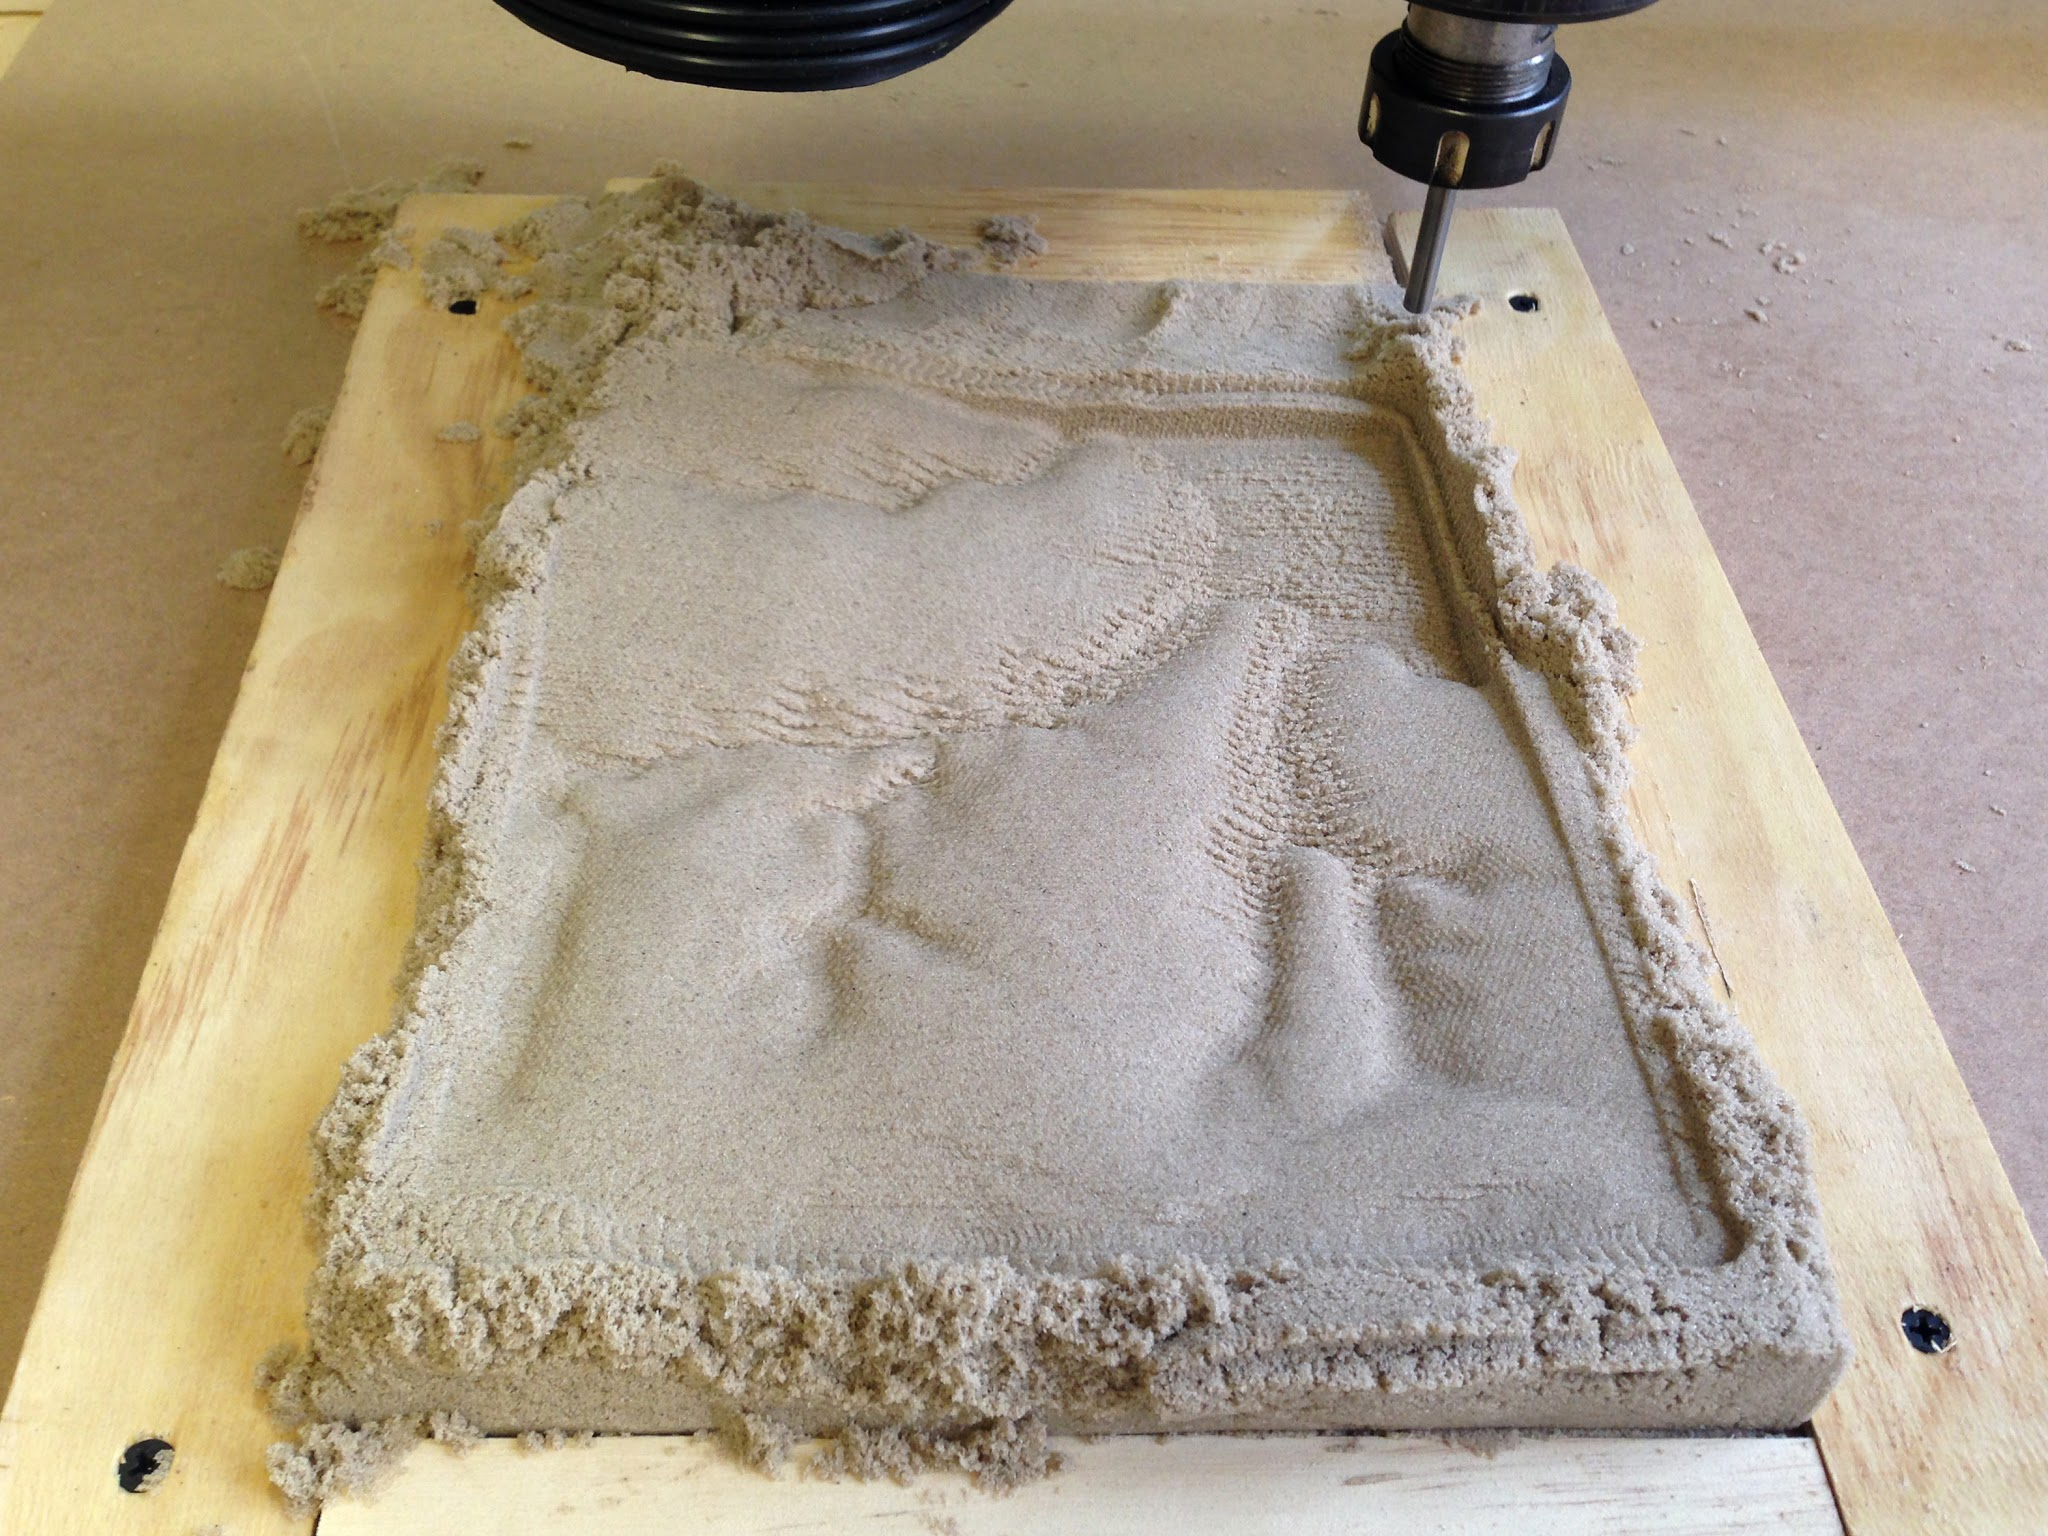
\includegraphics[width=\textwidth]{images/cnc_sand.jpg}
% \caption{{\bf Rapid prototyping.}
% 3-axis CNC fabrication of the evolved landscape in polymer-enriched sand using a plunge cut.}
% \label{fig:cnc_sand}
% \end{figure*}


% -------------- BIBLIOGRAPHY --------------

% \bibliographystyle{elsarticle-num}
 \bibliographystyle{elsarticle-harv}
% \bibliographystyle{elsarticle-num-names}
% \bibliographystyle{model1a-num-names}
% \bibliographystyle{model1b-num-names}
% \bibliographystyle{model1c-num-names}
% \bibliographystyle{model1-num-names}
% \bibliographystyle{model2-names}
% \bibliographystyle{model3a-num-names}
% \bibliographystyle{model3-num-names}
% \bibliographystyle{model4-names}
% \bibliographystyle{model5-names}
% \bibliographystyle{model6-num-names}

\bibliography{UASreview.bib}


\end{document}

